\section{규칙파 검증 실험 및 결과}

\subsection{조파기 구동 코드}

\begin{algorithm}[h]
    \caption{Sinusoidal Motion}
    \label{Sinusoidal Motion}
    \begin{algorithmic}[1]
    \Procedure{Sinusoidal Motion}{$A, N, \Delta\phi$}\Comment{Move the motor by sinusoidal function}
        \For{$elapsed Time \geq 0$}
            \If{$elapsed Time \geq N$}
                \State {$elapsed Time$ = 0}
                \State {$target = f(n)$}%\Comment{In this case, $target$ = $A \sin${($n$ $\Delta$$\phi$)}}
                % \State {$target$ = $A \sin${($n$ $\Delta$$\phi$)}}
                \State {$n$ $\gets$ $n$ + 1}
                \State {Move $motor$ to $target$}
            \EndIf
        \EndFor
        \EndProcedure
    \end{algorithmic}
\end{algorithm}

조파기 구동 코드는 시간간격 $N$마다 ($N$은 $\mathrm{~ms}$ 단위이다) 각 변위를 $f(n)$으로 지정하는 방식으로 작동한다 (알고리즘 \ref{Sinusoidal Motion}). 이 함수가 $\sin$형이면 모터가 사인형 각 변위를 따라 움직일 것으로 기대할 수 있다. sin형 구동을 위한 코드의 $f(n)$은 다음과 같다.
\begin{equation}
    f(n) = A \sin(n \Delta\phi)
    \label{f(n)}
\end{equation}

하지만 실질적인 매개변수는 $A, \omega, N$이며 $A$는 진폭, $\omega$는 조파판 위상의 각진동수, $N$은 조파판의 변위를 업데이트하는 시간 간격이다. $\omega$는 다음과 같이 정의될 수 있다.

\begin{equation}
    \omega = \frac{\Delta\phi}{\Delta t} = \frac{\Delta\phi}{N}, ~\Delta\phi = N \omega
    \label{f(N)}
\end{equation}

즉, $N$과 $\omega$가 매개된 입력 신호의 식을 알 수 있다. $A$와 $\omega$는 코드에서의 입력값과 조파기 구동 시 판의 움직임에서 실제로 나타나는 값이 달라 그 관계를 파악하기 위한 실험이 필수적이며, $\omega$를 크게 할 경우 탈조가 날 수 있어 가능 범위를 파악해야 한다. $N$은 이론적으로 조파판의 움직임에 영향을 주는 요소가 아니어서 이를 고정하여 실험을 진행했으나, 판의 최대 변위와 최소 변위 지점에서 변위가 업데이트되어야 하므로 각진동수에 따른 $N$의 변화가 필요할 수 있다. 즉, 각진동수의 크기에 따라서 최선의 $N$이 있을 수 있다는 것이다.

\subsection{예비 실험}
$A$는 $5\mathrm{~cm}$, $N$은 50으로 고정한 후, $\omega$를 $0.4\pi$에서 $\pi$까지 $0.1\pi$ 간격으로 변화시키며 실험하고 추가로 $1.5\pi$에 대해 실험을 진행하였다. 
이 경우 판의 움직임을 분석했을 때 $\omega$가 증가함에 따라 진폭의 출력값이 감소하는 것을 확인할 수 있었다. 생성되는 파의 경우, sin파 형태와 유사하고 각진동수는 입력값과 동일했지만 진폭은 관계가 없어서 실험 구성 단계에서는 모터의 움직임만 분석하기로 결정하였다. 

\subsection{실험 구성}
생성파의 분석이 필요치 않으므로 조파기의 모터 대신 작은 모터에 회로를 연결하여 모터의 움직임이 sin 형태인지를 확인하였다. 이는 시리얼 모니터에 현재 각 위치를 출력하여 알 수 있다. 각진동수의 출력값은 입력값과 일치하나 진폭은 달랐으며, $\omega$가 클수록 진폭의 출력값이 감소하였다 (그림 \ref{PreExperiment}).

\begin{figure}[H]
    \centering
    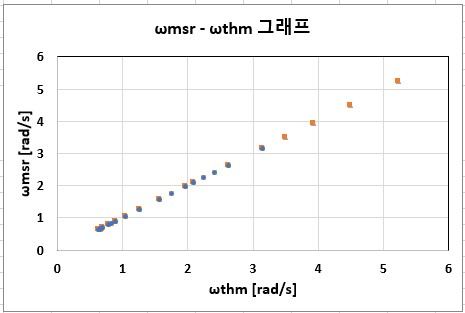
\includegraphics[height=5cm]{images/PreExperiment_Graph(Omega-Omega)-junlam.jpg}
    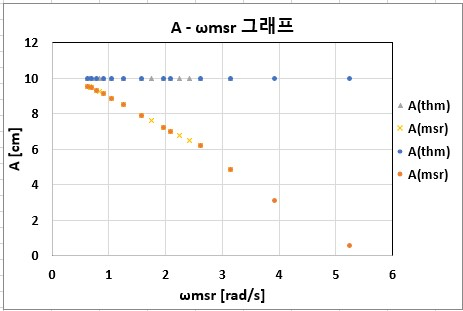
\includegraphics[height=5cm]{images/PreExperiment_Graph(A-Omega)-junlam.jpg}
    \caption{$\omega_{msr}$(측정값)에 대한 $\omega_{thm}$(입력값) (좌),  $\omega_{msr}$에 대한 진폭 $A_{msr}$(측정값) (우) - 예비 실험}
    \label{PreExperiment}
\end{figure}

그러므로 우리가 파를 생성하려고 할 때 구동 코드의 매개변수에 따른 판의 움직임과 생성되는 파 2개를 관찰해야 한다. 그리고 두 파의 진폭과 각진동수를 코드의 값과 비교하여 관계를 파악하는 것을 목표로 한다.

\begin{figure}[H]
    \centering
    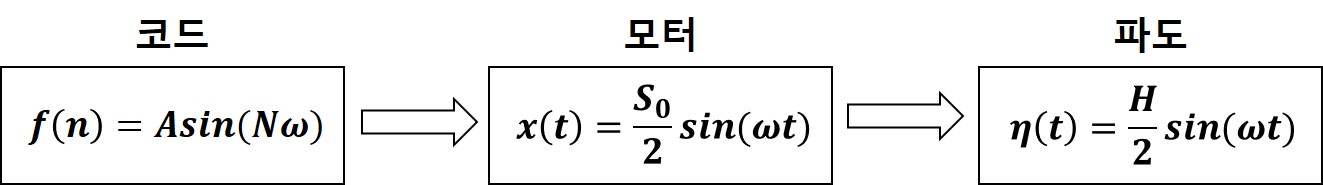
\includegraphics[width=12cm]{images/Flow_Chart(Analysis System_Kor).jpg}
    \caption{조파기 검증 실험의 흐름도}
    \label{Flow_Chart}
\end{figure}

비록 $S_0$와 $A$의 관계는 알 수 없으나 $S_0$와 $H$의 관계는 이론적 배경의 식을 따를 것으로 기대할 수 있으며 파가 sin형이 아니더라도 FFT 분석을 통해서 $\omega$를 구할 경우 세 파동에서 일관될 것이라고 예측할 수 있다.
이를 제대로 검증하기 위해서는 다양한 조건에 대한 데이터가 필요하며 이론적 분석과 예비 실험을 통해 정한 범위는 $A$는 $1\mathrm{~cm}$부터 $10\mathrm{~cm}$까지 $1\mathrm{~cm}$ 간격으로, $\omega$는 $3$부터 $12$까지 $1$ 간격으로 변화시키는 것이다. $N$은 50으로 고정시켰다 (단, 수심은 $15\mathrm{cm}$로 고정하였다).

%실험한 내용을 집어넣어야 함.

%실험계의 모식도가 필요함. 혹은 사진이라도.
\subsection{성능 검증 실험 결과}

\begin{figure}[H]
    \centering
    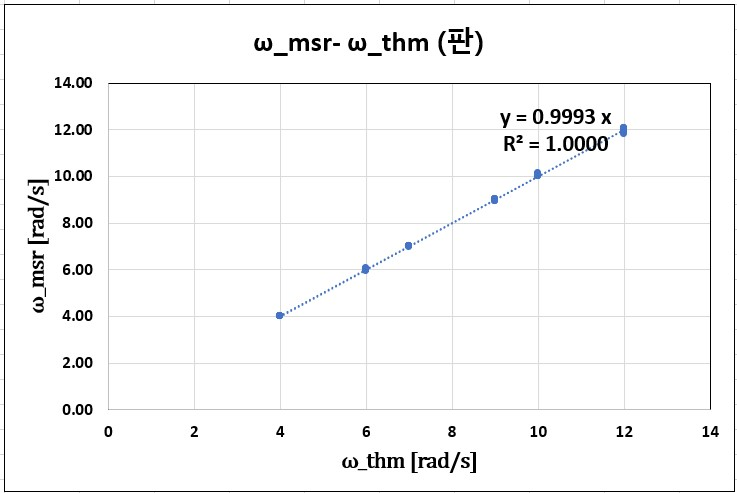
\includegraphics[height=5cm]{images/Experiment(omega_thm-omega_msr)_Plate_Kor.jpg}
    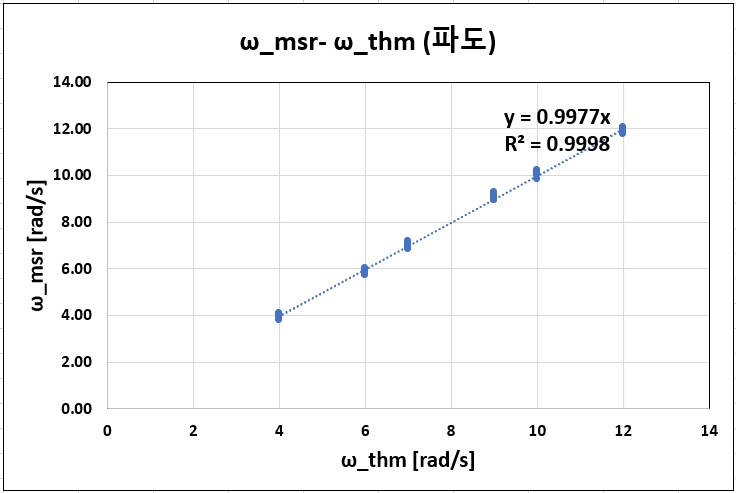
\includegraphics[height=5cm]{images/Experiment(omega_thm-omega_msr)_Wave_Kor.jpg}
    \caption{측정한 $\omega_{msr}$에 대한 코드의 $\omega_{thm}$ (좌),  $\omega_{msr}$에 대한 측정 진폭 $A_{msr}$ (우) - 검증 실험}
    \label{ExperimentGraph - 1, 2}
\end{figure}

그림 \ref{ExperimentGraph - 1, 2}에서 알 수 있듯이 $\omega$는 코드에서 대입한 값과 판, 파도 모두 같은 값을 띔을 알 수 있다 (두 그래프 모두 선형 관계를 만족하며($R^2 > 0.99$) 그 기울기는 약 1.000이다). 또, 분산 관계식과 식 \ref{eq:5}을 통해 주어진 $\omega$에 대한 $H/S$를 예측할 수 있고 이를 측정값과 비교해보았다 (그림 \ref{H/S Graph}).

\begin{figure}[H]
    \centering
    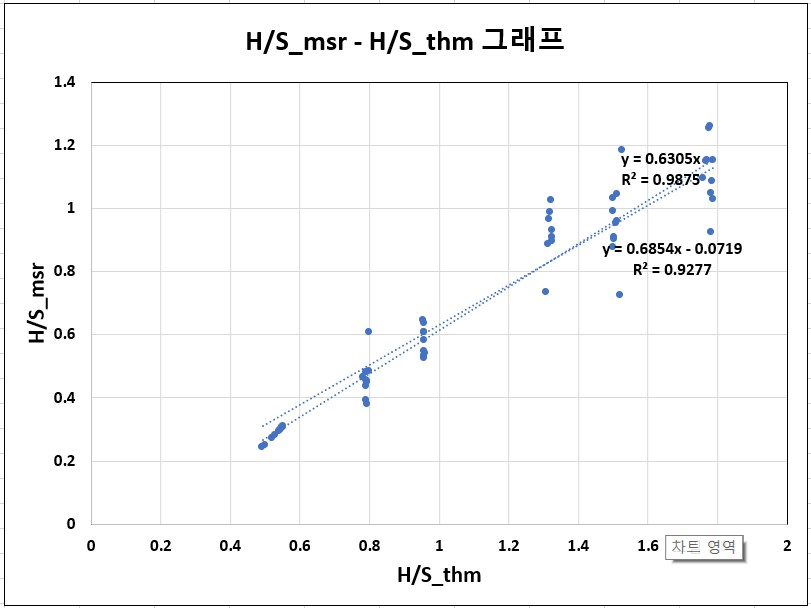
\includegraphics[width=0.70\textwidth]{images/Experiment(H.S_thm-H.S_msr).jpg}
    \caption{$H/S_{msr} - H/S_{thm}$ 그래프}
    \label{H/S Graph}
\end{figure}

$H/S$는 선형 관계를 만족한다고 볼 수 있다. 측정값이 구간으로 나타났으나 이는 불확도 내의 값으로 취급할 수 있으며 선형 추세선의 기울기가 $1.000$은 아니지만 선형 추세를 통해 매개변수로부터 $H/S$를 예측할 수 있다.

\begin{figure}[H]
    \centering
    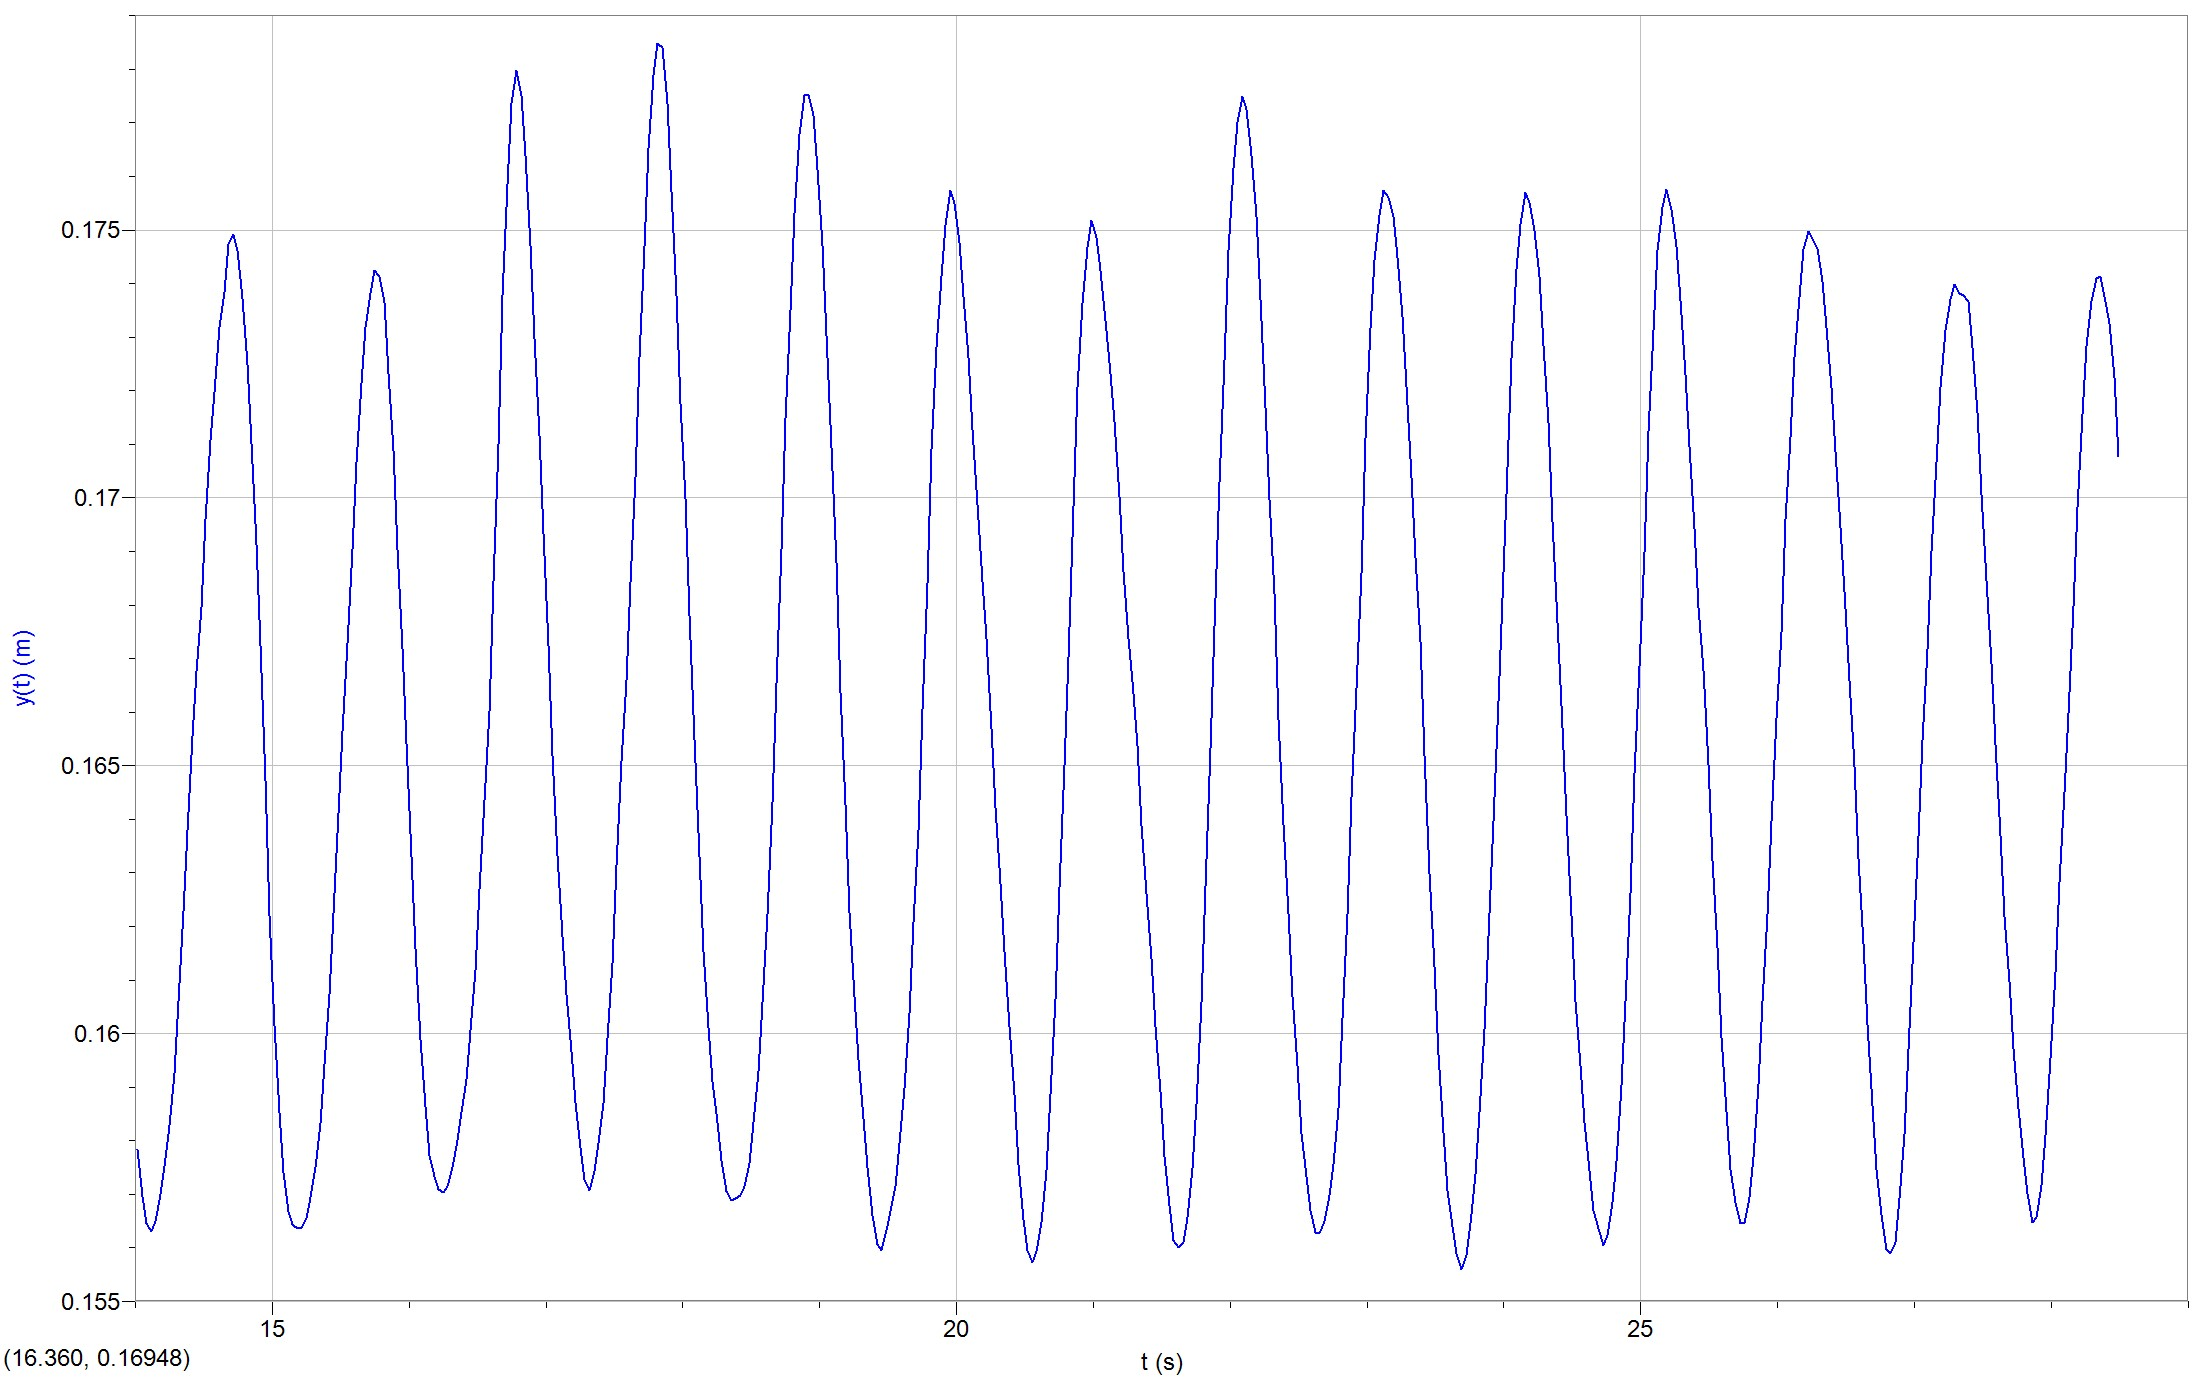
\includegraphics[width=0.70\textwidth]{images/Wave(omega=6,A=2).jpg}
    \caption{파형 데이터($A=2\mathrm{cm},~\omega=6\mathrm{rad/s}$)}
    \label{Example Wave Data}
\end{figure}

그림 \ref{Example Wave Data}는 한 sin 파의 예시이다. 코드에서는 $A=2\mathrm{cm},~\omega=6\mathrm{rad/s}$를 대입하였으며 측정값은 $A=0.9588\mathrm{cm},~\omega=5.959\mathrm{rad/s}$이다. 

\subsection{오차 원인}

본 실험에서는 실험 과정에서의 오차, 분석 상의 오차 등 여러 오차가 존재한다. 이는 크게 모터에 의한 것과 파고계 영상 분석에 의한 것으로 나눌 수 있다.

모터의 한계에 의한 것은 $\omega$에 따른 A의 한계와 아두이노에서 업로드한 파의 형태에 오차가 생기는 것이다. 최대 각가속도가 판 움직임의 진폭과 오차를 결정한다는 것은 실험을 통해 알 수 있었다. 실험은 $\omega = 6$, A = 5cm로 설정한 상태로, 각가속도만 $30,000\mathrm{step/s^2}, 40,000\mathrm{step/s^2}, 50,000\mathrm{step/s^2}$로 바꿔가며 판의 움직임을 조사하는 것으로 진행하였다. 이 때 판 움직임을 위상이 같도록 정렬한 결과가 아래의 그림이다. x축은 시간이고 y축은 판의 변위$(\mathrm{m})$이고 눈금 한 개의 스케일은 $0.01\mathrm{m}$이다.

\begin{figure}[H]
    \centering
    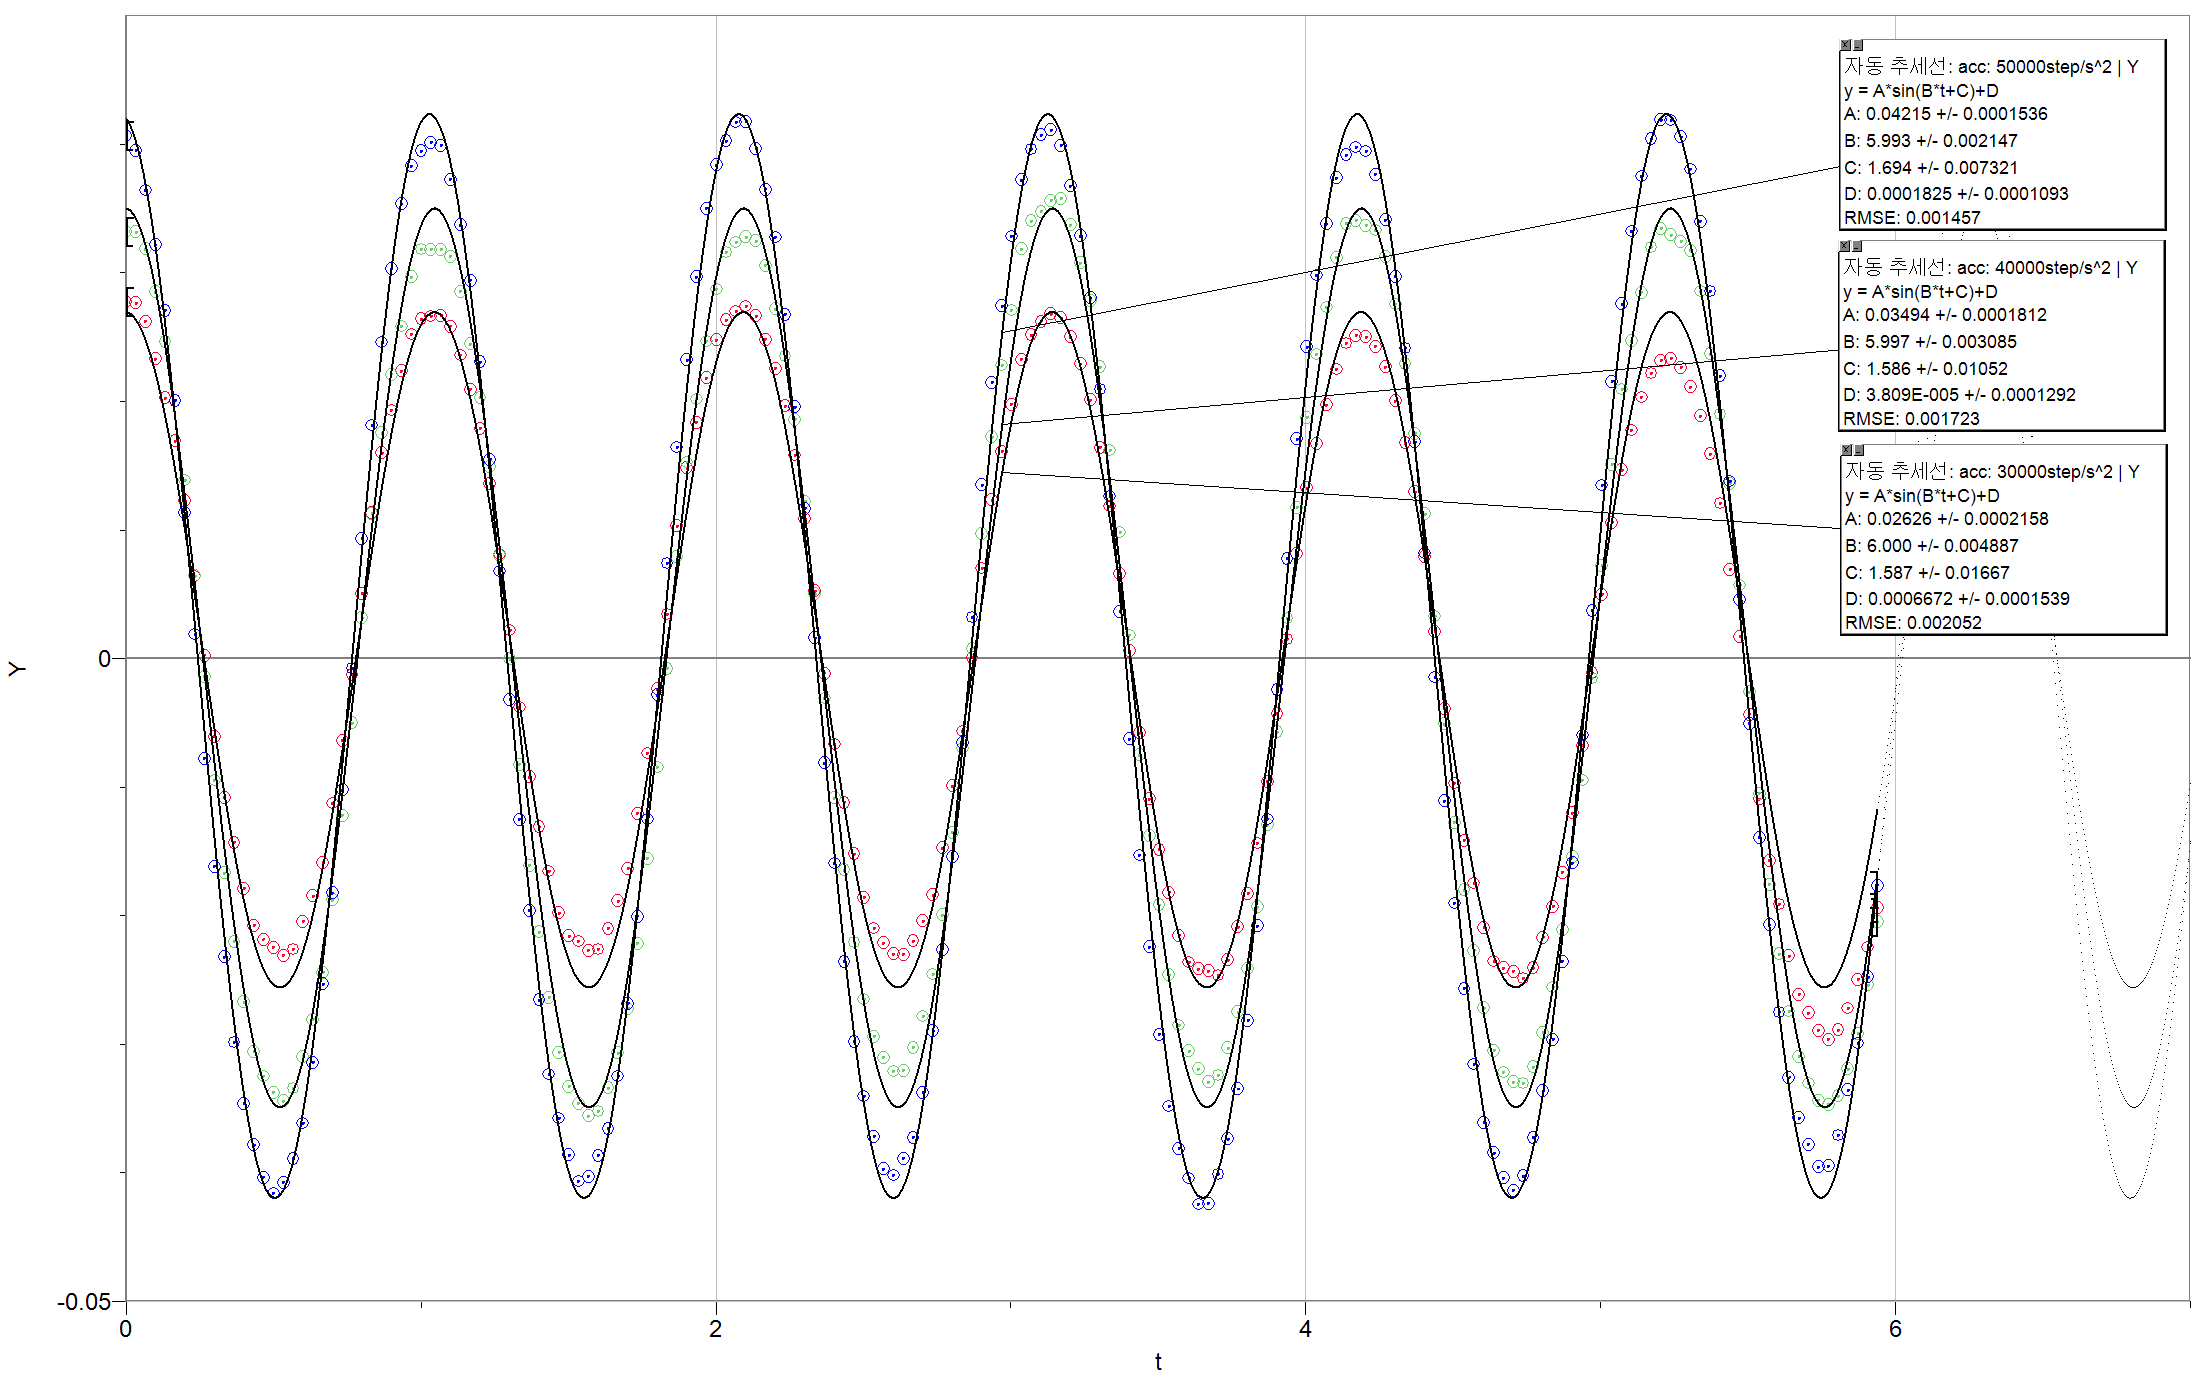
\includegraphics[width = 15cm, height = 10cm]{images/singraphofdiffacc.png}
    \caption{각가속도를 다르게 한 경우의 파고 데이터}
    \label{fig:enter-label}
\end{figure}
결과를 정리하면 각각은 다음과 같은 진폭과 진동수를 가진다.


\begin{table}[H]
    \centering
    \begin{tabular}{l|ll}
    \hline
    각가속도$(\mathrm{step/s^{2}})$ & $A (\mathrm{m})$ & RMSE \\
    \hline
    30,000 & 0.02626 & $2.052\times10^{-3}$ \\
    40,000 & 0.03494 & $1.723\times10^{-3}$ \\
    50,000 & 0.04215 & $1.457\times10^{-3}$\\
    \hline
    \end{tabular}%
\end{table}

해석하자면 목표한 진폭인 $5\mathrm{cm}$에 도달하지 못한 이유는 파의 구현에 필요한 각가속도가 $50,000\mathrm{step/s^2}$보다 크기 때문이라 볼 수 있는데, 물의 높이 $15\mathrm{cm}$를 기준으로 파가 중첩되어 생길 수 있는 최대 물의 높이에서 모터가 탈조나지 않기 위한 조건이 각가속도가 $30,000\mathrm{step/s^2}$ 이하일 것이기에 사용 중인 스텝모터로는 위의 $A-\omega$ 그래프에서 확인할 수 있는 정상적으로 구현되는 파만 구현 가능하다는 결론이 나온다.

%파도의 높낮이 변화가 극단적인 경우 부표식 파고계의 스티로폼 조각이 물 속에 잠겨버림->그로 인해서 진폭이 이론값보다 작게 나타남

%팽팽하게 위로 늘어났다가 풀리며 작은 마루가 옆에 생겨나는 현상도 관찰됨'

%쇄파 현상으로 인해 부표 위의 표식을 트래킹할 수 없

또, 본 실험에서는 스펀지와 유사한 재질의 포장재를 이용하여 얇은 직사각형판 모양의 부표를 만들었다. 이의 위치를 트래킹하여 파고를 측정하는데, 부표의 재질이 스펀지와 비슷하게 구멍이 많이 뚫려있는 재질이기에 파도의 높낮이 변화가 극단적일 경우, 물 위에 뜨지 못하고 잠시 잠기는 현상이 나타난다. 이로 인해 진폭이 이론값보다 작게 측정되는 오차가 있다. 또한 부표가 y축을 따라서만 움직이고 파도의 진행 방향에 영향을 받지 않도록 하기 위하여 부표에 두 개의 구멍을 뚫어 실을 통과시킨 후 이를 따라 움직이도록 하였는데, 마찰이 존재하므로 부표가 파도를 따라 위로 올라가는 과정에서 실이 늘어나게 된다. 실의 탄성에 의해 내려오는 과정에서 위로 튕기게 되어 파도의 큰 마루 옆에 작은 마루가 생기는 오차가 발생한다. 마지막으로, 쇄파 현상이 생기는 경우, 부표의 정중앙 표식이 부서지는 파도에 의해 가려져 정확히 같은 지점을 트래킹하는 것이 불가능하다.

%다 쓰면은 쌤한테 끝났다고 얘기하면 됨. 알겠냐?


\section{연구 결과 및 보고서 작성 지도}

\subsection{GS-touch 컨트롤러 하드웨어 제작}

Fig. \ref{fig:final_product_How_it_works_big}\는 최종 완성된 GS-touch 하드웨어와 GS-touch\가 동작하는 원리를  나타낸 것이다. PCB를 제작하여 부품을 하나하나 납땜하여 기판을 완성하였고, 3D 프린터를 이용하여 케이스를 출력하여 조립하였다. 전체적인 모양이나 크기 등 일부 개선할 부분이 있으나 사용하는데 큰 지장은 없다.

\begin{figure}[H]
	\begin{center}
		\begin{tikzpicture}
		\node[anchor=south west,inner sep=0] at (0,0) {\includegraphics[width=0.32\linewidth]{GS-touch_final} 
		\includegraphics[width=0.29\linewidth]{How_it_works_big}};
		\draw[text=black] (0.2, 7.3) node {(a)};
		\draw[text=black] (5.7, 7.3) node {(b)};
		\end{tikzpicture}
		\caption{(a) GS-touch 하드웨어와 (b) GS-touch 동작 원리}
	\label{fig:final_product_How_it_works_big}
	\end{center}
\end{figure}

\subsection{GS-touch 펌웨어 개발}

개발된 기반 펌웨어는 컴퓨터와 다르게 지정된 디스플레이어 에만 표시를 할 수 있다는 특징이 있다. 따라서 여러 가지 기능이 존재하더라도 한번에 여러 가지의 동작을 진행할 수는 없다. 그렇기 때문에 모터를 움직이는 여러 명령들을 효율적으로 처리하기 위해 하드웨어에 탑재된 버튼을 이용하여 이동과 선택이 쉬운 메뉴와 서브 메뉴를 만들어 사용하는 방식을 택하여 핵심 기능들이 모두 펌웨어에 들어갈 수 있도록 하였다.

\begin{figure}[h]
	\begin{center}
		\includegraphics[width=0.6\linewidth]{firmware_big}
	\end{center}
	\caption{펌웨어에 구현된 핵심 기능}
	\label{fig:firmware_big}
\end{figure}

펌웨어의 첫 번째 기능은 모터 초점 조절 장치의 핵심이라고도 할 수 있는 기능으로, 앞서 설명하였듯이 스테핑 모터를 조절하는 데 있어 가장 중요한 것은 정확한 스텝으로 정확한 각도를 이동하는 것이다. 즉, 제작한 펌웨어에는 현재 스테핑 모터의 각도를 나타내는 정보(position)를 나타낼 수 있으며, 버튼을 이용하여 아주 작은 간격(single step)으로 모터의 각도를 이동할 수 있도록 하였다.

장치를 사용하다보면 제공되는 최대 스텝수가 부족하거나 현재 위치를 기억해야 할 때가 있다. 이럴 때 필요한 기능이 position을 원하는 곳으로 초기화하는 것이다. 예를 들어, 대부분의 사람들은 포커서가 끝에 위치할 때의 position을 0으로 설정하고 싶을 것이다. 꼭 끝점이 아니더라도 이미 초점을 맞춘 상황을 기준으로 삼고 싶어서 position을 바꾸고 싶을 수 있을 것이다. 이 때 필요한 기능이 position을 지정된 범위 내에서 초기화시키는 것(reset position)이다. 위에서 설명한 상황이 아니더라도 GS-toufocuser을 껏다가 위치를 이동시켰던 경우에도 실제 위치를 기억하지 못할 때도 있을 것이다. 이런 상황에서도 position을 초기화시키는 기능이 사용될 것이다.

부가적인 기능으로, 망원경의 특성의 차이때문에 같은 각도를 이동하더라도 포커서가 이동하는 거리가 달라질 수도 있고, 필요한 힘이 달라지거나 한번에 이동하는 거리가 달라질 수도 있다. 이렇게 필요한 상황에 따라서 적절하게 microstepping을 바꿀 수 있는 기능 또한 펌웨어에 탑재되어있다. 또한, 모터를 움직이는 상황이 아니라면 센서에서 측정된 온도와 습도를 표시할 수 있도록 하였다.

\subsection{ASCOM driver 및 컨트롤 프로그램 개발}

ASCOM 드라이버를 ASCOM Protocol에 맞게 개발하여 여러가지 프로그램 및 망원경 사이의 편의성을 증대시키고자 하였다. ASCOM 드라이버는 직접 띄우는 창을 설정하여 여러가지 상황에 맞는 기능들을 제공할 수 있으며, 컴퓨터의 화면 상에서 일어나기 때문에 비교적 많은 정보를 한번에 표현할 수 있다.

C\#에서 지원하는 파일 형식은 .cs의 이름을 가지고 있으며, ASCOM Protocol에 맞게 작성된 ASCOM 드라이버를 표현하는 프로젝트는 크게 3가지 부분으로 이루어져 있다. Driver.cs 파일, SetupDialogForm.cs 파일, MainWindow.cs 파일이 그 세 가지이며, 각 파일들에서 실행시키는 영역이 모두 다르게 설계되어 있다.

Driver.cs는 serial Port를 이용하여 펌웨어와 직접적으로 통신하는 기능을 가지고 있다. ASCOM 지원 소프트웨어에서 장치를 구동하기 위해서 제일 먼저 해야 하는 일은 장치를 선택하고 통신환경 설정을 하는 것이다. Driver.cs는 ASCOM Setup을 선택할 경우 Fig. \ref{fig:focuserchooser}과 같이 나타나며 GS-touch ASCOM driver 이다. 이 드라이버가 설치되어 있지 않으면 GS-focus를 사용할 수 없다. 이 파일을 가장 중요한 기능은 프로그램이 내릴 수 있는 여러가지 명령을 serial command를 설정하여 각각 실행할 수 있도록 하는 것이다. 만약 서로 다른 프로그램에서 serial Port를 통한 연결(Port를 open한다고 표현한다)을 진행하려고 하면 그동안 진행했던 정보들을 모두 다시 전달해야하기 때문에 복잡한 처리과정을 거쳐야 한다. 때문에 serial Port와 관련된 함수 및 연결을 하나의 파일에서 모두 실행시킬 수 있도록 하였다.

\begin{figure}[h]
	\begin{center}
	\begin{tikzpicture}
	\node[anchor=south west,inner sep=0] at (0,0) {\includegraphics[width=0.6\linewidth]{focuserchooser}};
	\draw[draw=red, line width=0.5mm] (0.4, 2.05) rectangle (6.8, 2.61);
	\draw[text=red] (0.1, 2.3) node {(a)};
	\draw[draw=red, line width=0.5mm] (7.2, 2.05) rectangle (9.6, 2.61);
	\draw[text=red] (10.0, 2.30) node {(b)};
	\draw[draw=red, line width=0.5mm] (7.2, 1.04) rectangle (9.6, 1.55);
	\draw[text=red] (10.0, 1.29) node {(c)};
	\draw[draw=red, line width=0.5mm] (7.2, 0.33) rectangle (9.6, 0.84);
	\draw[text=red] (10.0, 0.58) node {(d)};
	\end{tikzpicture}
	\end{center}
	\caption{Focuser chooser windows : (a) choosing focuser, (b) Properties; excute SetupDialogForm.cs, (c) OK; apply results, (d) Cancel; close Form}
\label{fig:focuserchooser}	
\end{figure}

SetupDialogForm.cs는 ASCOM 드라이버를 선택하는 과정에서 직접적으로 연결을 진행하기 전에(직접적인 연결은 Connect를 눌러야 시작된다) 필요한 설정들을 확인하는 절차이다. 이 파일에서는 드라이버와 펌웨어 사이에 연결되어있는 COM port(serial 통신을 하기 위해 usb로 연결되어 있는 포트)를 지정하며, 모터의 microstepping을 설정한다. microstepping설정을 모터를 움직이는 도중에 직접 설정하게 되면 한 스텝당 이동하는 position이 달라지기 때문에 정확한 거리를 계산할 수 없게 되며, 측정을 한 번 진행할 때마다 Position 사이의 거리가 달라진다. 따라서 직접 연결을 진행하기 전에 microstepping을 다시 확인하게 된다.

\begin{figure}[h]
	\begin{center}
		\begin{tikzpicture}
		\node[anchor=south west,inner sep=0] at (0,0) {\includegraphics[width=0.6\linewidth]{setupdialogform_capture}};
		\draw[draw=red, line width=0.5mm] (0.4, 0.7) rectangle (3.20, 1.2);
		\draw[text=red] (0.10, 0.95) node {(a)};
		\draw[draw=red, line width=0.5mm] (0.4, 0.15) rectangle (3.2, 0.65);
		\draw[text=red] (0.10, 0.40) node {(b)};
		\draw[draw=red, line width=0.5mm] (9.8, 2.4) rectangle (6.4, 2.9);
		\draw[text=red] (10.2, 2.6) node {(c)};
		\draw[draw=red, line width=0.5mm] (9.8, 1.75) rectangle (6.4, 2.25);
		\draw[text=red] (10.2, 2.05) node {(d)};
		\draw[draw=red, line width=0.5mm] (7.8, 0.1) rectangle (5.65, 1.4);
		\draw[text=red] (5.3, 0.8) node {(e)};
		\draw[draw=red, line width=0.5mm] (9.8, 0.8) rectangle (8.0, 1.4);
		\draw[text=red] (10.2, 1.05) node {(f)};		
		\draw[draw=red, line width=0.5mm] (9.8, 0.1) rectangle (8.0, 0.7);
		\draw[text=red] (10.2, 0.35) node {(g)};		
		\end{tikzpicture}
	\end{center}
	\caption{SetupDialogForm : (a) show controller; checked show User Interface allows to show mainWindow when connected, (b) trace on; save log file (c) Reconnect; try to find COM Port, (c) COM Port; find TFocuser, (d) Microstepping; set Microstepping mode, (e) , (f) , (g) }
	\label{fig:setupdialogform_capture}	
\end{figure}



MainWindow.cs는 직접 연결을 실행했을 때 우리 눈에 직접 들어오는 컨트롤 창의 정보에 대한 파일이다. MainWindow의 버튼들은 각각 펌웨어에서 설정한 serialcommand와 연결되어있어 버튼이 눌릴 때마다 Driver.cs에서 serialcommand를 통해 자료를 주고받으며, 새로 업데이트된 정보는 다시 MainWindow 창에 표시되는 작업이 반복되게 된다. 

\begin{figure}[h]
	\begin{subfigure}{0.5\textwidth}
		\begin{center}
			\includegraphics[width=0.75\linewidth]{mainwindow1} 
		\end{center}	
		\caption{Running appearance}
		\label{fig:mainwindow1}
	\end{subfigure}
	\begin{subfigure}{0.5\textwidth}
		\begin{center}			
			\includegraphics[width=0.75\linewidth]{mainwindow2}
		\end{center}
		\caption{Advanced Running appearance}
		\label{fig:mainwindow2}
	\end{subfigure}
	\caption{MainWindow.cs가 실행되었을 때의 모습}
	\label{fig:mainwindow}
\end{figure}

MainWindow.cs는 펌웨어보다 자유로운 설정이 가능하기 때문에 보다 많은 기능들을 탑재할 수 있었다. 기본적인 기능인 스텝당 움직이는 기능과 더불어 한번에 이동할 single step을 얼마나 크게 할지 직접 설정할 수 있고, 원한다면 모터를 그 상태에서 정지시킬 수도 있으며, 원하는 position을 입력하면 모터가 그 position으로 자동으로 이동하게 할 수도 있다(Move to). 부가적으로는 microstepping과 온도 및 습도를 실시간으로 확인할 수 있으며, 모터가 움직이는 속도와 가속도를 범위 내에서 직접 설정할 수도 있다.

직접 개발한 펌웨어에서도 여러 장점을 찾을 수 있다. Micro Touch제품의 경우, 앞서 나열한 것 외에도 스텝의 초기화 기능이 없기 때문에 모터제어기를 끄고 망원경을 컨트롤하는 등의 변수가 생기면 그 전으로 돌아가기 어렵게 된다. 또한 자신이 원하는 스텝의 위치로 바로 옮기는 것 또한 어려운데, 이 드라이버에서는 원하는 position으로 바로 이동하는 기능도 지원하고 있다. 


\subsection{\LaTeX\를 이용한 보고서 작성}

\LaTeX\은 문서 조판에 사용되는 프로그램이다. 도널드 커누스가 만든 \TeX\을 쉽게 사용하기 위하여 1984년에 레슬리 램포트가 만든 매크로이다. \TeX\을 직접 사용하기는 어렵기 때문에, 오늘날에는 \LaTeX\을 이용하여 문서를 만드는 경우가 많다. 연구 보고서, 작품 설명서 등을 작성하기 위해 \LaTeX\를 사용하였데 처음 진입 장벽이 높아 처음 학생을 지도할 때는 조금 시간이 걸렸다. 하지만 코딩을 좋아하는 학생은 익숙해 지고 나서 오히려 지도교사인 나보다 더 잘 사용을 한다는 느낌이 든다. \LaTeX\은 다음과 같은 장점이 있어 연구 보고서 작성이나 논문 작성에 편리하다. 

\begin{itemize}
\item 문서가 예쁘고 깔끔하다.
\item 수식 편집이 편하고 빠르다.
\item labeling과 referencing이 편하다.
\item ToC, LoF, LoT 등이 자동화되어 있다.
\item Vector 이미지를 쉽게 삽입할 수 있다.
\item 호환이 잘 된다.
\item 초기 설정을 완료한 후에는 형식에 신경쓸 필요가 없다.
\item 디자인보다 내용에 집중할 수 있다.
\item 다양한 패키지가 존재한다.
\end{itemize}	


